\subsubsection*{Т4}


Выясним полноты некоторых систем функций в пространстве $L_2[0,\pi/2]$. Начём с 
\begin{equation*}
    \{f_n(x) = \sin[(2n-1)x]\}_{n\in \mathbb{N}}.
\end{equation*}

\begin{to_def}
    Пусть $X$ -- нормированное пространство. Система $S = \{f_\alpha\}_{\alpha\in \mathcal A}$ называется \textit{полной}, если $\forall x \in X$ $\forall \varepsilon > 0$ $\exists \alpha_1, \ldots, \alpha_n \in \mathcal A$, а также $\exists f_{\alpha_1}, \ldots, f_{\alpha_n} \in S$ такие, что $\|x- (\alpha_1 f_{\alpha_1} + \ldots + \alpha_n f_{\alpha_n})\|_X < \varepsilon$.
\end{to_def}

Стоит подчеркнуть, что это не определение базиса, так как $\alpha \equiv \alpha(\varepsilon)$. Это определение слабее базиса, это -- приближение.

Если мы возьмём $L_2[-\pi,\pi]$, и систему вида $\{1, \sin(nx), \cos(nx)\}_{n\in \mathbb{N}}$, то она будет полна, более того будет являеться базисом. В рамках задачи мы интересуемся промежутком $[0, \pi/2]$. 

Более того, такая система полна в $\overset{\circ}{C}[-\pi, \pi],\, (f(-\pi)=f(\pi))$, чем мы потом воспользуемся в Т5.

В смысле $L_2$ мы можем приближать, игнорируя счётное число точек:
\begin{equation*}
    \|f-\tau_n\|_2^2 = \int_0^{\pi/2} |f-\tau_n| (x) \mu(\d x).
\end{equation*}
Достраивая функцию специфичным образом на отрезок $[-\pi, \pi]$ (u, d, u, d), пользуемся знанием о полноте тригонометрической системы и приходим к полной системе. 

Для понимания продолжения функции с отрезка $[0, \pi/2]$, на $[-\pi, \pi]$, достаточно построить функции, образующие системы (рис. 1). 
\begin{figure}[ht]
    \centering
    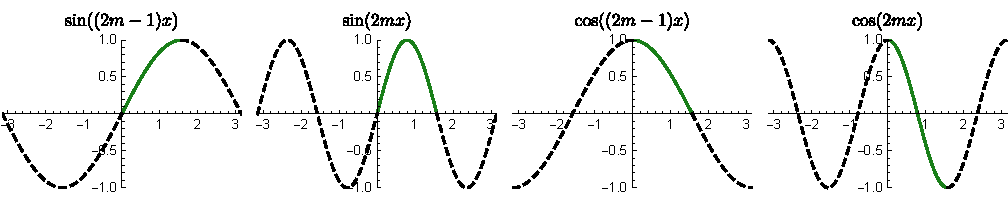
\includegraphics[width=0.8\textwidth]{figures/1.pdf}
    \caption{Графики функция при $m=1$ для Т4}
\end{figure}
И, аналогично, для $k=2$ (рис. 2). 
\begin{figure}[ht]
    \centering
    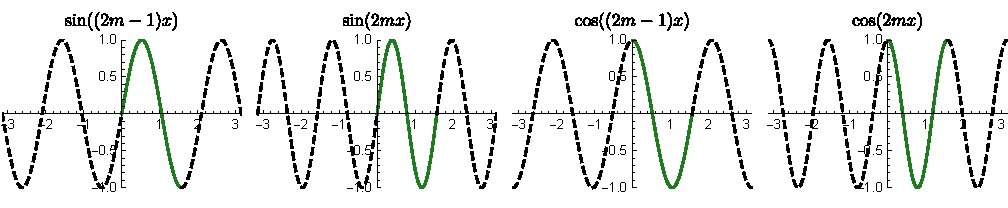
\includegraphics[width=0.8\textwidth]{figures/2.pdf}
    \caption{Графики функция при $m=2$ для Т4}
\end{figure}



